\documentclass[utf8x,xcolor=dvipsnames]{beamer}
%\documentclass[utf8x,xcolor=dvipsnames]{beamer}
%\documentclass[utf8x,handout]{beamer}

%\usetheme{Darmstadt}

%\usetheme{default}
%\usetheme{Boadilla}
%\usetheme{CambridgeUS} 
%\usetheme{Pittsburgh}
\usetheme{Rochester}

%NOPE
%\usetheme{Warsaw}
%\usetheme{Bergen}
%\usetheme{AnnArbor}

\usecolortheme[RGB={173,27,1}]{structure}
%\usecolortheme[named=Brown]{structure}



\newcommand{\code}[1]{\texttt{#1}}

\usefonttheme[onlylarge]{structurebold}
\useoutertheme{infolines} 
\setbeamerfont*{frametitle}{size=\normalsize,series=\bfseries}
%\setbeamertemplate{navigation symbols}{}
\setbeamertemplate{navigation symbols}{}

%to get rid of the ``()'' in the footbar.
    \defbeamertemplate*{footline}{my infolines theme}
    {
      \leavevmode%
      \hbox{%
      \begin{beamercolorbox}[wd=.333333\paperwidth,ht=2.25ex,dp=1ex,center]{author in head/foot}%
        \usebeamerfont{author in head/foot}\insertshortinstitute
      \end{beamercolorbox}%
      \begin{beamercolorbox}[wd=.333333\paperwidth,ht=2.25ex,dp=1ex,center]{title in head/foot}%
        \usebeamerfont{title in head/foot}\insertshorttitle
      \end{beamercolorbox}%
      \begin{beamercolorbox}[wd=.333333\paperwidth,ht=2.25ex,dp=1ex,right]{date in head/foot}%
        \usebeamerfont{date in head/foot}\insertshortdate{}\hspace*{2em}
        \insertframenumber{} / \inserttotalframenumber\hspace*{2ex}
      \end{beamercolorbox}}%
      \vskip0pt%
    }



%\setbeamertemplate{footline}{\hspace*{.5cm}\scriptsize{\insertshorttitle
%\hspace*{50pt} \hfill\insertframenumber\hspace*{.5cm}}\\
%\vspace{9pt}} 
%\usepackage[utf8]{inputenc}

%\usepackage{cancel}
%\usepackage{listings}

\usepackage{fancyvrb}
\usepackage{color}
%\usepackage[utf-8]{inputenc}



\makeatletter
\def\PYG@reset{\let\PYG@it=\relax \let\PYG@bf=\relax%
    \let\PYG@ul=\relax \let\PYG@tc=\relax%
    \let\PYG@bc=\relax \let\PYG@ff=\relax}
\def\PYG@tok#1{\csname PYG@tok@#1\endcsname}
\def\PYG@toks#1+{\ifx\relax#1\empty\else%
    \PYG@tok{#1}\expandafter\PYG@toks\fi}
\def\PYG@do#1{\PYG@bc{\PYG@tc{\PYG@ul{%
    \PYG@it{\PYG@bf{\PYG@ff{#1}}}}}}}
\def\PYG#1#2{\PYG@reset\PYG@toks#1+\relax+\PYG@do{#2}}

\def\PYG@tok@gd{\def\PYG@tc##1{\textcolor[rgb]{0.63,0.00,0.00}{##1}}}
\def\PYG@tok@gu{\let\PYG@bf=\textbf\def\PYG@tc##1{\textcolor[rgb]{0.50,0.00,0.50}{##1}}}
\def\PYG@tok@gt{\def\PYG@tc##1{\textcolor[rgb]{0.00,0.25,0.82}{##1}}}
\def\PYG@tok@gs{\let\PYG@bf=\textbf}
\def\PYG@tok@gr{\def\PYG@tc##1{\textcolor[rgb]{1.00,0.00,0.00}{##1}}}
\def\PYG@tok@cm{\let\PYG@it=\textit\def\PYG@tc##1{\textcolor[rgb]{0.25,0.50,0.56}{##1}}}
\def\PYG@tok@vg{\def\PYG@tc##1{\textcolor[rgb]{0.73,0.38,0.84}{##1}}}
\def\PYG@tok@m{\def\PYG@tc##1{\textcolor[rgb]{0.13,0.50,0.31}{##1}}}
\def\PYG@tok@mh{\def\PYG@tc##1{\textcolor[rgb]{0.13,0.50,0.31}{##1}}}
\def\PYG@tok@cs{\def\PYG@tc##1{\textcolor[rgb]{0.25,0.50,0.56}{##1}}\def\PYG@bc##1{\colorbox[rgb]{1.00,0.94,0.94}{##1}}}
\def\PYG@tok@ge{\let\PYG@it=\textit}
\def\PYG@tok@vc{\def\PYG@tc##1{\textcolor[rgb]{0.73,0.38,0.84}{##1}}}
\def\PYG@tok@il{\def\PYG@tc##1{\textcolor[rgb]{0.13,0.50,0.31}{##1}}}
\def\PYG@tok@go{\def\PYG@tc##1{\textcolor[rgb]{0.19,0.19,0.19}{##1}}}
\def\PYG@tok@cp{\def\PYG@tc##1{\textcolor[rgb]{0.00,0.44,0.13}{##1}}}
\def\PYG@tok@gi{\def\PYG@tc##1{\textcolor[rgb]{0.00,0.63,0.00}{##1}}}
\def\PYG@tok@gh{\let\PYG@bf=\textbf\def\PYG@tc##1{\textcolor[rgb]{0.00,0.00,0.50}{##1}}}
\def\PYG@tok@ni{\let\PYG@bf=\textbf\def\PYG@tc##1{\textcolor[rgb]{0.84,0.33,0.22}{##1}}}
\def\PYG@tok@nl{\let\PYG@bf=\textbf\def\PYG@tc##1{\textcolor[rgb]{0.00,0.13,0.44}{##1}}}
\def\PYG@tok@nn{\let\PYG@bf=\textbf\def\PYG@tc##1{\textcolor[rgb]{0.05,0.52,0.71}{##1}}}
\def\PYG@tok@no{\def\PYG@tc##1{\textcolor[rgb]{0.38,0.68,0.84}{##1}}}
\def\PYG@tok@na{\def\PYG@tc##1{\textcolor[rgb]{0.25,0.44,0.63}{##1}}}
\def\PYG@tok@nb{\def\PYG@tc##1{\textcolor[rgb]{0.00,0.44,0.13}{##1}}}
\def\PYG@tok@nc{\let\PYG@bf=\textbf\def\PYG@tc##1{\textcolor[rgb]{0.05,0.52,0.71}{##1}}}
\def\PYG@tok@nd{\let\PYG@bf=\textbf\def\PYG@tc##1{\textcolor[rgb]{0.33,0.33,0.33}{##1}}}
\def\PYG@tok@ne{\def\PYG@tc##1{\textcolor[rgb]{0.00,0.44,0.13}{##1}}}
\def\PYG@tok@nf{\def\PYG@tc##1{\textcolor[rgb]{0.02,0.16,0.49}{##1}}}
\def\PYG@tok@si{\let\PYG@it=\textit\def\PYG@tc##1{\textcolor[rgb]{0.44,0.63,0.82}{##1}}}
\def\PYG@tok@s2{\def\PYG@tc##1{\textcolor[rgb]{0.25,0.44,0.63}{##1}}}
\def\PYG@tok@vi{\def\PYG@tc##1{\textcolor[rgb]{0.73,0.38,0.84}{##1}}}
\def\PYG@tok@nt{\let\PYG@bf=\textbf\def\PYG@tc##1{\textcolor[rgb]{0.02,0.16,0.45}{##1}}}
\def\PYG@tok@nv{\def\PYG@tc##1{\textcolor[rgb]{0.73,0.38,0.84}{##1}}}
\def\PYG@tok@s1{\def\PYG@tc##1{\textcolor[rgb]{0.25,0.44,0.63}{##1}}}
\def\PYG@tok@gp{\let\PYG@bf=\textbf\def\PYG@tc##1{\textcolor[rgb]{0.78,0.36,0.04}{##1}}}
\def\PYG@tok@sh{\def\PYG@tc##1{\textcolor[rgb]{0.25,0.44,0.63}{##1}}}
\def\PYG@tok@ow{\let\PYG@bf=\textbf\def\PYG@tc##1{\textcolor[rgb]{0.00,0.44,0.13}{##1}}}
\def\PYG@tok@sx{\def\PYG@tc##1{\textcolor[rgb]{0.78,0.36,0.04}{##1}}}
\def\PYG@tok@bp{\def\PYG@tc##1{\textcolor[rgb]{0.00,0.44,0.13}{##1}}}
\def\PYG@tok@c1{\let\PYG@it=\textit\def\PYG@tc##1{\textcolor[rgb]{0.25,0.50,0.56}{##1}}}
\def\PYG@tok@kc{\let\PYG@bf=\textbf\def\PYG@tc##1{\textcolor[rgb]{0.00,0.44,0.13}{##1}}}
\def\PYG@tok@c{\let\PYG@it=\textit\def\PYG@tc##1{\textcolor[rgb]{0.25,0.50,0.56}{##1}}}
\def\PYG@tok@mf{\def\PYG@tc##1{\textcolor[rgb]{0.13,0.50,0.31}{##1}}}
\def\PYG@tok@err{\def\PYG@bc##1{\fcolorbox[rgb]{1.00,0.00,0.00}{1,1,1}{##1}}}
\def\PYG@tok@kd{\let\PYG@bf=\textbf\def\PYG@tc##1{\textcolor[rgb]{0.00,0.44,0.13}{##1}}}
\def\PYG@tok@ss{\def\PYG@tc##1{\textcolor[rgb]{0.32,0.47,0.09}{##1}}}
\def\PYG@tok@sr{\def\PYG@tc##1{\textcolor[rgb]{0.14,0.33,0.53}{##1}}}
\def\PYG@tok@mo{\def\PYG@tc##1{\textcolor[rgb]{0.13,0.50,0.31}{##1}}}
\def\PYG@tok@mi{\def\PYG@tc##1{\textcolor[rgb]{0.13,0.50,0.31}{##1}}}
\def\PYG@tok@kn{\let\PYG@bf=\textbf\def\PYG@tc##1{\textcolor[rgb]{0.00,0.44,0.13}{##1}}}
\def\PYG@tok@o{\def\PYG@tc##1{\textcolor[rgb]{0.40,0.40,0.40}{##1}}}
\def\PYG@tok@kr{\let\PYG@bf=\textbf\def\PYG@tc##1{\textcolor[rgb]{0.00,0.44,0.13}{##1}}}
\def\PYG@tok@s{\def\PYG@tc##1{\textcolor[rgb]{0.25,0.44,0.63}{##1}}}
\def\PYG@tok@kp{\def\PYG@tc##1{\textcolor[rgb]{0.00,0.44,0.13}{##1}}}
\def\PYG@tok@w{\def\PYG@tc##1{\textcolor[rgb]{0.73,0.73,0.73}{##1}}}
\def\PYG@tok@kt{\def\PYG@tc##1{\textcolor[rgb]{0.56,0.13,0.00}{##1}}}
\def\PYG@tok@sc{\def\PYG@tc##1{\textcolor[rgb]{0.25,0.44,0.63}{##1}}}
\def\PYG@tok@sb{\def\PYG@tc##1{\textcolor[rgb]{0.25,0.44,0.63}{##1}}}
\def\PYG@tok@k{\let\PYG@bf=\textbf\def\PYG@tc##1{\textcolor[rgb]{0.00,0.44,0.13}{##1}}}
\def\PYG@tok@se{\let\PYG@bf=\textbf\def\PYG@tc##1{\textcolor[rgb]{0.25,0.44,0.63}{##1}}}
\def\PYG@tok@sd{\let\PYG@it=\textit\def\PYG@tc##1{\textcolor[rgb]{0.25,0.44,0.63}{##1}}}

\def\PYGZbs{\char`\\}
\def\PYGZus{\char`\_}
\def\PYGZob{\char`\{}
\def\PYGZcb{\char`\}}
\def\PYGZca{\char`\^}
\def\PYGZsh{\char`\#}
\def\PYGZpc{\char`\%}
\def\PYGZdl{\char`\$}
\def\PYGZti{\char`\~}
% for compatibility with earlier versions
\def\PYGZat{@}
\def\PYGZlb{[}
\def\PYGZrb{]}
\makeatother

\definecolor{VerbatimColor}{rgb}{0.97,0.97,0.97} % light gray
\definecolor{VerbatimBorderColor}{rgb}{0,0,0} %black


\newenvironment{mycode}
{\VerbatimEnvironment
% \captionof{example}{#2}\ifx\relax#1\relax\else\label{#1}\fi%
\begin{SaveVerbatim}[commandchars=\\\{\}, fontsize=\tiny]{SVerbEnv}}
{\end{SaveVerbatim}\fcolorbox{VerbatimBorderColor}{VerbatimColor}{\parbox{\textwidth}{\scriptsize \BUseVerbatim{SVerbEnv}}}}

%\usepackage{fancyhdr}
\usepackage{fancyvrb}
\usepackage{color}
\usepackage{listings}

\lstset{%
basicstyle=\footnotesize,
language=C++,
backgroundcolor=\color{lightgray},
frame=single,
tabsize=2,
breaklines=true,
showspaces=false,
showstringspaces=false,
%framexleftmargin=5mm, frame=shadowbox, rulesepcolor=\color{blue}
}
% Redefine these colors to something not white if you want to have colored
% background and border for code examples.
\definecolor{VerbatimColor}{rgb}{0.97,0.97,0.97} % light gray
\definecolor{VerbatimBorderColor}{rgb}{0,0,0} %black

% Redefine the Verbatim environment to allow border and background colors.
% The original environment is still used for verbatims within tables.
\let\OriginalVerbatim=\Verbatim
\let\endOriginalVerbatim=\endVerbatim

% Play with vspace to be able to keep the indentation.
\newlength\distancetoright
\def\mycolorbox#1{%
  \setlength\distancetoright{\linewidth}%
  \advance\distancetoright -\@totalleftmargin %
  \fcolorbox{VerbatimBorderColor}{VerbatimColor}{%
  \begin{minipage}{\distancetoright}%
    #1
  \end{minipage}%
  }%
}
\def\FrameCommand{\mycolorbox}

\renewcommand{\Verbatim}[1][1]{%
  % list starts new par, but we don't want it to be set apart vertically
  \bgroup\parskip=0pt%
  \smallskip%
  % The list environement is needed to control perfectly the vertical
  % space.
  \list{}{%
  \setlength\parskip{0pt}%
  \setlength\itemsep{0ex}%
  \setlength\topsep{0ex}%
  \setlength\partopsep{0pt}%
  \setlength\leftmargin{0pt}%
  }%
  \item\MakeFramed {\FrameRestore}%
     \small%
    \OriginalVerbatim[#1]%
}
\renewcommand{\endVerbatim}{%
    \endOriginalVerbatim%
  \endMakeFramed%
  \endlist%
  % close group to restore \parskip
  \egroup%
}


\newcommand{\code}[1]{\texttt{#1}}



% Setup TikZ
\usepackage[normalem]{ulem}
\usepackage{tikz}
\usetikzlibrary{arrows}
\tikzstyle{block}=[draw opacity=0.7,line width=1.4cm]

% Author, Title, etc.
\titlegraphic{\center \pgfimage[height=1.5cm]{images/google}}

\title[First steps with or-tools] 
{%
  Chapter~2: First steps with or-tools:\\ cryptarithmetic puzzles%
}
\subtitle{or-tools library}
\author
{
  Nikolaj van Omme%\inst{1}
  \and%
  Laurent Perron%
}
\institute[Google]{}
%\institute
%{
  %Google

%}

\date{\today}

\pgfdeclareimage[height=0.6cm]{logo}{images/logo}
\logo{\pgfuseimage{logo}}

\begin{document}

\begin{frame}
  \titlepage
\end{frame}

\begin{frame}[shrink]{Overview:}%[allowframebreaks]
  \tableofcontents
\end{frame}

\begin{frame}{Before we start~\ldots}
  \begin{itemize}
    \item<1-> \textbf{Prerequisites:}
    \begin{itemize}
      \item<2-> Some basic knowledge of C++.
      \item<3-> Some basic knowledge of Constraint Programming.
    \end{itemize}
\vspace{1cm}
    \item<4-> \textbf{Code:} \uncover<5->{(\code{documentation/tutorials/C++/chap2})}
    \begin{itemize}
      \item<6-> \code{cp\_is\_fun1.cc}: A simple cryptarithmetic puzzle.
      \item<7-> \code{cp\_is\_fun2.cc}: Use of \code{SolutionCollector}s to collect some or all solutions.
      \item<8-> \code{cp\_is\_fun3.cc}: Use of the \href{http://code.google.com/p/gflags/}{Google gflags library} to parse command line parameters.
      \item<9-> \code{cp\_is\_fun4.cc}: Use of parameters.
    \end{itemize}
  \end{itemize}
\end{frame}

\section{The problem and a first model}

\subsection{Description of the problem}






\begin{frame}[fragile]
\frametitle{CP is Fun!}
 \begin{columns}
 \begin{column}{0.15\textwidth}
\begin{uncoverenv}<2->
  \begin{verbatim}
      C P
+     I S
+   F U N
---------
= T R U E
  \end{verbatim}
\end{uncoverenv}
 \end{column}
\begin{column}{0.70\textwidth}
 \begin{itemize}
      \item<1-> A simple cryptarithmetic puzzle.
      \item<3-> A feasible solution:\\ \code{C=2 P=3 I=7 S=4 F=9 U=6 N=8 T=1 R=0 E=5}
      \item<4-> Indeed: \code{23+74+968 = 1065}
      \item<5-> 72 solutions! \uncover<6->{\color{red}{In base 10!}}
    \end{itemize}
 \end{column}
 \begin{column}{0.15\textwidth}
\begin{uncoverenv}<4->
  \begin{verbatim}
      2 3
+     7 4
+   9 6 8
---------
= 1 0 6 5
  \end{verbatim}
\end{uncoverenv}
 \end{column}
\end{columns}
\end{frame}

\begin{frame}{Three-stage method}
  \begin{itemize}
    \item<1-> \textbf{Describe:}
    \begin{itemize}
      \item<4-> Goal of the puzzle?\\ \uncover<5->{replace letters by digits such that \code{CP+IS+FUN=TRUE}}
      \item<6-> What are the unknowns?\\ \uncover<7->{one letter = one variable}
      \item<8-> What are the constraints?\\ 
	\begin{itemize}
	  \item<9-> sum has to be verified
	  \item<10-> two different letters represent two different digits
	  \item<11-> first digit of a number can not be 0
	  \item<12-> \alt<12>{10 letters: we need at least 10 different digits}{\sout{10 letters: we need at least 10 different digits}}
	\end{itemize}

    \end{itemize}

    \item<2-> \textbf{Model:}
    \begin{itemize}
      \item<14-> Given a base $\mathtt{b}$, digits range from $0$ to $\mathtt{b}-1$
      \item<15-> ${\color{blue}{\mathtt{C}}} \cdot \mathtt{b}+{\color{blue}{\mathtt{P}}}+{\color{blue}{\mathtt{I}}} \cdot \mathtt{b}+{\color{blue}{\mathtt{S}}}+{\color{blue}{\mathtt{F}}} \cdot \mathtt{b}^2 +
{\color{blue}{\mathtt{U}}} \cdot \mathtt{b} + {\color{blue}{\mathtt{N}}} = {\color{blue}{\mathtt{T}}} \cdot \mathtt{b}^3 + {\color{blue}{\mathtt{R}}} \cdot \mathtt{b}^2 + {\color{blue}{\mathtt{U}}} \cdot \mathtt{b}
+ {\color{blue}{\mathtt{E}}}$.
      \item<16-> \code{AllDifferent(C,P,I,S,F,U,N,T,R,E)}
      \item<17-> $\mathtt{C, I, F, T} \in [1,\mathtt{b}-1]$ and $\mathtt{P, S, U, N, R, E} \in [0,\mathtt{b}-1]$



    
    \end{itemize}
\item<3-> \textbf{Solve:} \uncover<18->{Later~\ldots}
  \end{itemize}
\end{frame}

\section{Anatomy of a basic C++ code}
\subsection{At a glance}

\begin{frame}[shrink]{At a glance}
 \begin{columns}
 \begin{column}{0.45\textwidth}
 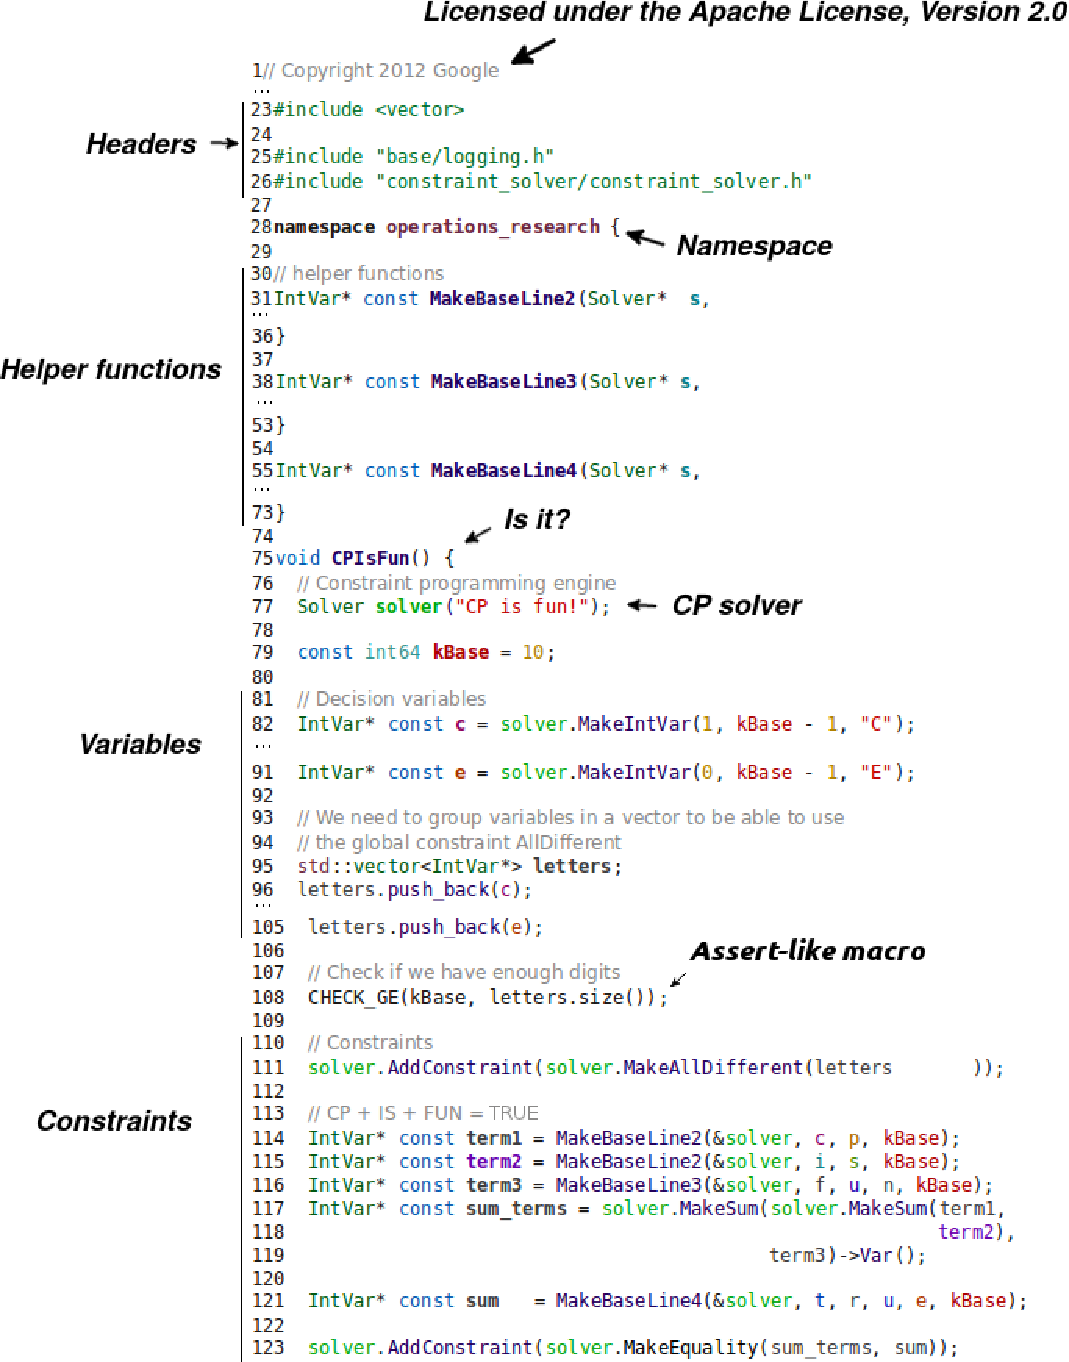
\includegraphics[height=0.9\textheight]{images/anatomy1.pdf}
\end{column}
 \begin{column}{0.45\textwidth}
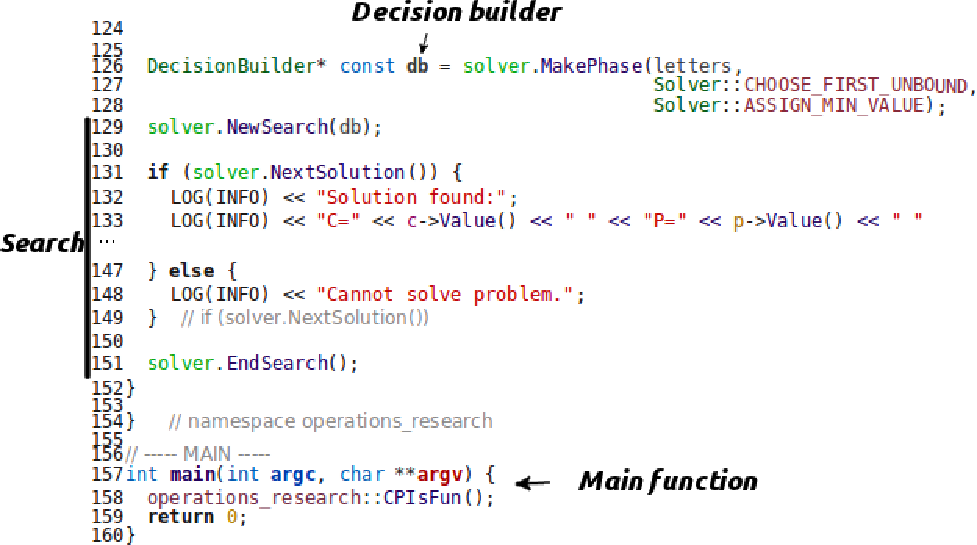
\includegraphics[height=95pt]{images/anatomy2.pdf}
\end{column}
\end{columns}
\end{frame}

\subsection{Headers}

\begin{frame}[fragile]{Headers}
 
To use the library, we need to include a few headers:\\
~\\
\begin{uncoverenv}<2->
\begin{mycode}
#include "base/logging.h"
#include "constraint_solver/constraint_solver.h"
\end{mycode}
\end{uncoverenv}
~\\
~\\
\begin{itemize}
 \item<3-> \code{logging.h}: logging facilities and some assert-like macros.
 \item<4-> \code{constraint\_solver.h}: main entry point to the CP solver.

 
\end{itemize}

\end{frame}


\subsection{The namespace \texttt{operations\_research}}


\begin{frame}[fragile]{The namespace \code{operations\_research}}
 
The whole library is nested in the namespace \code{operations\_research}:
\medskip
\begin{uncoverenv}<2->
\begin{mycode}
\PYG{k}{namespace} \PYG{n}{operations\PYGZus{}research} \PYG{p}{\PYGZob{}}
  \PYG{n}{IntVar}\PYG{o}{*} \PYG{k}{const} \PYG{n}{MakeBaseLine2}\PYG{p}{(}\PYG{p}{.}\PYG{p}{.}\PYG{p}{.}\PYG{p}{)} \PYG{p}{\PYGZob{}}
    \PYG{p}{.}\PYG{p}{.}\PYG{p}{.}
  \PYG{p}{\PYGZcb{}}
  \PYG{p}{.}\PYG{p}{.}\PYG{p}{.}
  \PYG{k+kt}{void} \PYG{n}{CPIsFun}\PYG{p}{(}\PYG{p}{)} \PYG{p}{\PYGZob{}}
    \PYG{c+c1}{// Magic happens here!}
  \PYG{p}{\PYGZcb{}}
\PYG{p}{\PYGZcb{}}  \PYG{c+c1}{// namespace operations\PYGZus{}research}
\end{mycode}
\end{uncoverenv}

\medskip

\uncover<3->{\code{CPIsFun()} is where all the magic happens:}
\medskip
\begin{uncoverenv}<4->
\begin{mycode}
\PYG{k+kt}{int} \PYG{n}{main}\PYG{p}{(}\PYG{k+kt}{int} \PYG{n}{argc}\PYG{p}{,} \PYG{k+kt}{char} \PYG{o}{*}\PYG{o}{*}\PYG{n}{argv}\PYG{p}{)} \PYG{p}{\PYGZob{}}
  \PYG{n}{operations\PYGZus{}research}\PYG{o}{:}\PYG{o}{:}\PYG{n}{CPIsFun}\PYG{p}{(}\PYG{p}{)}\PYG{p}{;}
  \PYG{k}{return} \PYG{l+m+mi}{0}\PYG{p}{;}
\PYG{p}{\PYGZcb{}}
\end{mycode}
\end{uncoverenv}

\end{frame}

\subsection{The CP solver}

\begin{frame}[fragile]{The Constraint Programming (CP) solver}
 
The CP solver:

\begin{itemize}
 \item<2-> is the main engine to solve an instance;
 \item<3-> is responsible for the creation of the model;
 \item<4-> has a very rich Application Programming Interface (API) and
 \item<5-> provides a lots of functionalities.
\end{itemize}
\vspace{0.5cm}
\uncover<6->{The CP solver is created as follows:}

\medskip

\begin{uncoverenv}<7->
\begin{mycode}
Solver solver("CP is fun!");
\end{mycode}
\end{uncoverenv}

\end{frame}

\subsection{Variables}

\begin{frame}[fragile]{The decision variables}
To create the decision variables:
\medskip
\begin{uncoverenv}<2->
\begin{mycode}
\PYG{k}{const} \PYG{n}{int64} \PYG{n}{kBase} \PYG{o}{=} \PYG{l+m+mi}{10}\PYG{p}{;}
\PYG{n}{IntVar}\PYG{o}{*} \PYG{k}{const} \PYG{n}{c} \PYG{o}{=} \PYG{n}{solver}\PYG{p}{.}\PYG{n}{MakeIntVar}\PYG{p}{(}\PYG{l+m+mi}{1}\PYG{p}{,} \PYG{n}{kBase} \PYG{o}{-} \PYG{l+m+mi}{1}\PYG{p}{,} \PYG{l+s}{"}\PYG{l+s}{C}\PYG{l+s}{"}\PYG{p}{)}\PYG{p}{;}
\PYG{n}{IntVar}\PYG{o}{*} \PYG{k}{const} \PYG{n}{p} \PYG{o}{=} \PYG{n}{solver}\PYG{p}{.}\PYG{n}{MakeIntVar}\PYG{p}{(}\PYG{l+m+mi}{0}\PYG{p}{,} \PYG{n}{kBase} \PYG{o}{-} \PYG{l+m+mi}{1}\PYG{p}{,} \PYG{l+s}{"}\PYG{l+s}{P}\PYG{l+s}{"}\PYG{p}{)}\PYG{p}{;}
\PYG{p}{.}\PYG{p}{.}\PYG{p}{.}
\PYG{n}{IntVar}\PYG{o}{*} \PYG{k}{const} \PYG{n}{e} \PYG{o}{=} \PYG{n}{solver}\PYG{p}{.}\PYG{n}{MakeIntVar}\PYG{p}{(}\PYG{l+m+mi}{0}\PYG{p}{,} \PYG{n}{kBase} \PYG{o}{-} \PYG{l+m+mi}{1}\PYG{p}{,} \PYG{l+s}{"}\PYG{l+s}{E}\PYG{l+s}{"}\PYG{p}{)}\PYG{p}{;}
\end{mycode}
\end{uncoverenv}
\uncover<3->{%
\begin{block}{Factory methods in or-tools}
The solver API provides
numerous factory methods to create different objects. These methods
start with \code{Make} and return a pointer to the newly created object.

The solver automatically takes  ownership of these objects and deletes
them appropriately.
\end{block}%
}

\uncover<4->{
\begin{alertblock}{Warning:}
 Never delete explicitly an object created by a factory method!
\end{alertblock}
}
\end{frame}

\subsection{Assert-like macros}
\begin{frame}[fragile]
\frametitle{Program defensively!}
\begin{itemize}
 \item<2-> Assert-like macros are defined in the header \code{logging.h}.
 \item<3-> Base has to be at greater than or equal to 10:
\end{itemize}

\begin{uncoverenv}<4->
\begin{mycode}
\PYG{n}{CHECK\PYGZus{}GE}\PYG{p}{(}\PYG{n}{kBase}\PYG{p}{,} \PYG{n}{letters}\PYG{p}{.}\PYG{n}{size}\PYG{p}{(}\PYG{p}{)}\PYG{p}{)}\PYG{p}{;}
\end{mycode}
\end{uncoverenv}

\begin{itemize}
 \item<5-> \code{CHECK\_GE(x,y)} checks if condition (x) \textgreater{}= (y) is true.
 \item<6-> If not, the program is aborted and the cause is printed:
\end{itemize}

\begin{uncoverenv}<6->
\begin{mycode}
[23:51:34] examples/cp\_is\_fun1.cc:108: Check failed:
                                             (kBase) \textgreater{}= (letters.size())
Aborted
\end{mycode}
\end{uncoverenv}

\end{frame}

\subsection{Constraints}
\begin{frame}[fragile]
\frametitle{Constraints I}
To multiply an integer variable with an integer constant:
\medskip
\begin{uncoverenv}<2->
\begin{mycode}
\PYG{n}{IntVar}\PYG{o}{*} \PYG{k}{const} \PYG{n}{var1} \PYG{o}{=} \PYG{n}{solver}\PYG{p}{.}\PYG{n}{MakeIntVar}\PYG{p}{(}\PYG{l+m+mi}{0}\PYG{p}{,} \PYG{l+m+mi}{1}\PYG{p}{,} \PYG{l+s}{"}\PYG{l+s}{Var1}\PYG{l+s}{"}\PYG{p}{)}\PYG{p}{;}
\PYG{n}{IntVar}\PYG{o}{*} \PYG{k}{const} \PYG{n}{var2} \PYG{o}{=} \PYG{n}{solver}\PYG{p}{.}\PYG{n}{MakeProd}\PYG{p}{(}\PYG{n}{var1}\PYG{p}{,}\PYG{l+m+mi}{36}\PYG{p}{)}\PYG{o}{-}\PYG{o}{\textgreater{}}\PYG{n}{Var}\PYG{p}{(}\PYG{p}{)}\PYG{p}{;}
\end{mycode}
\end{uncoverenv}

\medskip
\uncover<3->{To add two IntVar given by their respective pointers:}
\medskip

\begin{uncoverenv}<4->
\begin{mycode}
\PYG{n}{IntVar}\PYG{o}{*} \PYG{k}{const} \PYG{n}{var3} \PYG{o}{=} \PYG{n}{solver}\PYG{p}{.}\PYG{n}{MakeSum}\PYG{p}{(}\PYG{n}{var1}\PYG{p}{,}\PYG{n}{var2}\PYG{p}{)}\PYG{o}{-}\PYG{o}{\textgreater{}}\PYG{n}{Var}\PYG{p}{(}\PYG{p}{)}\PYG{p}{;}
\end{mycode}
\end{uncoverenv}

\uncover<5->{
\begin{alertblock}{Warning:}
Never store a pointer to an \code{IntExpr} nor a \code{BaseIntExpr} in the code. The safe code should always call \code{Var()} on an expression built by the solver, and store the object as an \code{IntVar*}.
\end{alertblock}
}

\end{frame}

\begin{frame}[fragile]
\frametitle{Constraints II}
\sloppy
\makebox{To construct a sum, we use a combination of \code{MakeSum()} and \code{MakeProd()}} factory methods:
\medskip
\begin{uncoverenv}<2->
\begin{mycode}
\PYG{n}{IntVar}\PYG{o}{*} \PYG{k}{const} \PYG{n}{term1} \PYG{o}{=} \PYG{n}{solver}\PYG{p}{.}\PYG{n}{MakeSum}\PYG{p}{(}\PYG{n}{solver}\PYG{p}{.}\PYG{n}{MakeProd}\PYG{p}{(}\PYG{n}{c}\PYG{p}{,}\PYG{n}{kBase}\PYG{p}{)}\PYG{p}{,}\PYG{n}{p}\PYG{p}{)}\PYG{o}{-}\PYG{o}{\textgreater{}}\PYG{n}{Var}\PYG{p}{(}\PYG{p}{)}\PYG{p}{;}
\end{mycode}
\end{uncoverenv}

\medskip
\uncover<3->{If the number of terms in the sum to construct is large, you can use \code{MakeScalProd()}:}
\medskip

\begin{uncoverenv}<4->
\begin{mycode}
\PYG{n}{IntVar}\PYG{o}{*} \PYG{k}{const} \PYG{n}{var1} \PYG{o}{=} \PYG{n}{solver}\PYG{p}{.}\PYG{n}{MakeInt}\PYG{p}{(}\PYG{p}{.}\PYG{p}{.}\PYG{p}{.}\PYG{p}{)}\PYG{p}{;}
\PYG{p}{.}\PYG{p}{.}\PYG{p}{.}
\PYG{n}{IntVar}\PYG{o}{*} \PYG{k}{const} \PYG{n}{varN} \PYG{o}{=} \PYG{n}{solver}\PYG{p}{.}\PYG{n}{MakeInt}\PYG{p}{(}\PYG{p}{.}\PYG{p}{.}\PYG{p}{.}\PYG{p}{)}\PYG{p}{;}
\PYG{n}{std}\PYG{o}{:}\PYG{o}{:}\PYG{n}{vector}\PYG{o}{\textless{}}\PYG{n}{IntVar}\PYG{o}{*}\PYG{o}{\textgreater{}} \PYG{n}{variables}\PYG{p}{;}
\PYG{n}{variables}\PYG{p}{.}\PYG{n}{push\PYGZus{}back}\PYG{p}{(}\PYG{n}{var1}\PYG{p}{)}\PYG{p}{;}
\PYG{p}{.}\PYG{p}{.}\PYG{p}{.}
\PYG{n}{variables}\PYG{p}{.}\PYG{n}{push\PYGZus{}back}\PYG{p}{(}\PYG{n}{varN}\PYG{p}{)}\PYG{p}{;}

\PYG{n}{std}\PYG{o}{:}\PYG{o}{:}\PYG{n}{vector}\PYG{o}{\textless{}}\PYG{n}{int64}\PYG{o}{\textgreater{}} \PYG{n}{coefficients}\PYG{p}{(}\PYG{n}{N}\PYG{p}{)}\PYG{p}{;}
\PYG{c+c1}{// fill vector with coefficients}
\PYG{p}{.}\PYG{p}{.}\PYG{p}{.}
\PYG{n}{IntVar}\PYG{o}{*} \PYG{k}{const} \PYG{n}{sum} \PYG{o}{=} \PYG{n}{solver}\PYG{p}{.}\PYG{n}{MakeScalProd}\PYG{p}{(}\PYG{n}{variables}\PYG{p}{,} \PYG{n}{coefficients}\PYG{p}{)}\PYG{o}{-}\PYG{o}{\textgreater{}}\PYG{n}{Var}\PYG{p}{(}\PYG{p}{)}\PYG{p}{;}
\end{mycode}
\end{uncoverenv}


\end{frame}

\begin{frame}[fragile]
\frametitle{Constraints III}
\sloppy
\makebox{To create the sum constraint, we use the factory method~\code{MakeEquality()}} that returns a pointer
to a \code{Constraint} object:
\medskip
\begin{uncoverenv}<2->
\begin{mycode}
\PYG{n}{IntVar}\PYG{o}{*} \PYG{k}{const} \PYG{n}{term1} \PYG{o}{=} \PYG{p}{.}\PYG{p}{.}\PYG{p}{.}
\PYG{n}{IntVar}\PYG{o}{*} \PYG{k}{const} \PYG{n}{term2} \PYG{o}{=} \PYG{p}{.}\PYG{p}{.}\PYG{p}{.}
\PYG{n}{IntVar}\PYG{o}{*} \PYG{k}{const} \PYG{n}{term3} \PYG{o}{=} \PYG{p}{.}\PYG{p}{.}\PYG{p}{.}

\PYG{n}{IntVar}\PYG{o}{*} \PYG{k}{const} \PYG{n}{sum\PYGZus{}terms} \PYG{o}{=} \PYG{n}{solver}\PYG{p}{.}\PYG{n}{MakeSum}\PYG{p}{(}\PYG{n}{solver}\PYG{p}{.}\PYG{n}{MakeSum}\PYG{p}{(}\PYG{n}{term1}\PYG{p}{,}
                                                        \PYG{n}{term2}\PYG{p}{)}\PYG{p}{,}
                                         \PYG{n}{term3}\PYG{p}{)}\PYG{o}{-}\PYG{o}{\textgreater{}}\PYG{n}{Var}\PYG{p}{(}\PYG{p}{)}\PYG{p}{;}
\PYG{n}{IntVar}\PYG{o}{*} \PYG{k}{const} \PYG{n}{sum} \PYG{o}{=} \PYG{p}{.}\PYG{p}{.}\PYG{p}{.}

\PYG{n}{Constraint}\PYG{o}{*} \PYG{k}{const} \PYG{n}{sum\PYGZus{}constraint} \PYG{o}{=} \PYG{n}{solver}\PYG{p}{.}\PYG{n}{MakeEquality}\PYG{p}{(}\PYG{n}{sum\PYGZus{}terms}\PYG{p}{,} \PYG{n}{sum}\PYG{p}{)}\PYG{p}{;}
\end{mycode}
\end{uncoverenv}

\medskip
\uncover<3->{To add a constraint:}
\medskip

\begin{uncoverenv}<4->
\begin{mycode}
\PYG{n}{solver}\PYG{p}{.}\PYG{n}{AddConstraint}\PYG{p}{(}\PYG{n}{sum\PYGZus{}constraint}\PYG{p}{)}\PYG{p}{;}
\end{mycode}
\end{uncoverenv}

\vspace{0.3cm}
\uncover<5->{or:}
\smallskip
\begin{uncoverenv}<6->
\begin{mycode}
\PYG{n}{solver}\PYG{p}{.}\PYG{n}{AddConstraint}\PYG{p}{(}\PYG{n}{solver}\PYG{p}{.}\PYG{n}{MakeEquality}\PYG{p}{(}\PYG{n}{sum\PYGZus{}terms}\PYG{p}{,} \PYG{n}{sum}\PYG{p}{)}\PYG{p}{)}\PYG{p}{;}
\end{mycode}
\end{uncoverenv}
\end{frame}


\begin{frame}[fragile]
\frametitle{Constraints IV}
The global \code{AllDifferent} constraint:
\medskip
\begin{uncoverenv}<2->
\begin{mycode}
\PYG{n}{std}\PYG{o}{:}\PYG{o}{:}\PYG{n}{vector}\PYG{o}{\textless{}}\PYG{n}{IntVar}\PYG{o}{*}\PYG{o}{\textgreater{}} \PYG{n}{letters}\PYG{p}{;}
\PYG{n}{letters}\PYG{p}{.}\PYG{n}{push\PYGZus{}back}\PYG{p}{(}\PYG{n}{c}\PYG{p}{)}\PYG{p}{;}
\PYG{n}{letters}\PYG{p}{.}\PYG{n}{push\PYGZus{}back}\PYG{p}{(}\PYG{n}{p}\PYG{p}{)}\PYG{p}{;}
\PYG{p}{.}\PYG{p}{.}\PYG{p}{.}
\PYG{n}{letters}\PYG{p}{.}\PYG{n}{push\PYGZus{}back}\PYG{p}{(}\PYG{n}{e}\PYG{p}{)}\PYG{p}{;}

\PYG{n}{solver}\PYG{p}{.}\PYG{n}{AddConstraint}\PYG{p}{(}\PYG{n}{solver}\PYG{p}{.}\PYG{n}{MakeAllDifferent}\PYG{p}{(}\PYG{n}{letters}\PYG{p}{)}\PYG{p}{)}\PYG{p}{;}
\end{mycode}
\end{uncoverenv}


\end{frame}

\subsection{The Decision Builder}

\begin{frame}[fragile]
\frametitle{The Decision Builder}
A \code{DecisionBuilder} is responsible for creating the actual search tree.
\medskip
\begin{uncoverenv}<2->
\begin{mycode}
\PYG{n}{DecisionBuilder}\PYG{o}{*} \PYG{k}{const} \PYG{n}{db} \PYG{o}{=} \PYG{n}{solver}\PYG{p}{.}\PYG{n}{MakePhase}\PYG{p}{(}\PYG{n}{letters}\PYG{p}{,}
                                          \PYG{n}{Solver}\PYG{o}{:}\PYG{o}{:}\PYG{n}{CHOOSE\PYGZus{}FIRST\PYGZus{}UNBOUND}\PYG{p}{,}
                                          \PYG{n}{Solver}\PYG{o}{:}\PYG{o}{:}\PYG{n}{ASSIGN\PYGZus{}MIN\PYGZus{}VALUE}\PYG{p}{)}\PYG{p}{;}
\end{mycode}
\end{uncoverenv}

\medskip
\uncover<3->{Parameters of the method \code{MakePhase}:}
\medskip
\begin{itemize}
 \item<4-> \code{letters}: \code{std::vector} with pointers to the \code{IntVar} decision variables.
 \item<5-> \code{Solver::CHOOSE\_FIRST\_UNBOUND}: next selected \code{IntVar} variable in the search is the first unbounded variable.
 \item<6-> \code{Solver::ASSIGN\_MIN\_VALUE}: assign the smallest available value to the selected \code{IntVar}.
\end{itemize}

\end{frame}

\subsection{The search and the solutions}

\begin{frame}[fragile]
\frametitle{The search I}
To prepare for a new search:
\medskip
\begin{uncoverenv}<2->
\begin{mycode}
\PYG{n}{DecisionBuilder}\PYG{o}{*} \PYG{k}{const} \PYG{n}{db} \PYG{o}{=} \PYG{p}{.}\PYG{p}{.}\PYG{p}{.}
\PYG{n}{solver}\PYG{p}{.}\PYG{n}{NewSearch}\PYG{p}{(}\PYG{n}{db}\PYG{p}{)}\PYG{p}{;}
\end{mycode}
\end{uncoverenv}

\medskip
\uncover<3->{To actually search for the next solution in the search tree:}
\medskip
\begin{uncoverenv}<4->
\begin{mycode}
\PYG{k}{if} \PYG{p}{(}\PYG{n}{solver}\PYG{p}{.}\PYG{n}{NextSolution}\PYG{p}{(}\PYG{p}{)}\PYG{p}{)} \PYG{p}{\PYGZob{}}
  \PYG{c+c1}{// Do something with the current solution}
\PYG{p}{\PYGZcb{}} \PYG{k}{else} \PYG{p}{\PYGZob{}}
  \PYG{c+c1}{// The search is finished}
\PYG{p}{\PYGZcb{}}
\end{mycode}
\end{uncoverenv}

\end{frame}

\begin{frame}[fragile]
\frametitle{The search II}
We print out the found solution and check if it is valid:
\medskip
\begin{uncoverenv}<2->
\begin{mycode}
\PYG{k}{if} \PYG{p}{(}\PYG{n}{solver}\PYG{p}{.}\PYG{n}{NextSolution}\PYG{p}{(}\PYG{p}{)}\PYG{p}{)} \PYG{p}{\PYGZob{}}
  \PYG{n}{LOG}\PYG{p}{(}\PYG{n}{INFO}\PYG{p}{)} \PYG{o}{\textless{}}\PYG{o}{\textless{}} \PYG{l+s}{"}\PYG{l+s}{Solution found:}\PYG{l+s}{"}\PYG{p}{;}
  \PYG{n}{LOG}\PYG{p}{(}\PYG{n}{INFO}\PYG{p}{)} \PYG{o}{\textless{}}\PYG{o}{\textless{}} \PYG{l+s}{"}\PYG{l+s}{C=}\PYG{l+s}{"} \PYG{o}{\textless{}}\PYG{o}{\textless{}} \PYG{n}{c}\PYG{o}{-}\PYG{o}{\textgreater{}}\PYG{n}{Value}\PYG{p}{(}\PYG{p}{)} \PYG{o}{\textless{}}\PYG{o}{\textless{}} \PYG{l+s}{"}\PYG{l+s}{ }\PYG{l+s}{"} \PYG{o}{\textless{}}\PYG{o}{\textless{}} \PYG{l+s}{"}\PYG{l+s}{P=}\PYG{l+s}{"} \PYG{o}{\textless{}}\PYG{o}{\textless{}} \PYG{n}{p}\PYG{o}{-}\PYG{o}{\textgreater{}}\PYG{n}{Value}\PYG{p}{(}\PYG{p}{)} \PYG{o}{\textless{}}\PYG{o}{\textless{}} \PYG{l+s}{"}\PYG{l+s}{ }\PYG{l+s}{"}
            \PYG{o}{\textless{}}\PYG{o}{\textless{}} \PYG{l+s}{"}\PYG{l+s}{I=}\PYG{l+s}{"} \PYG{o}{\textless{}}\PYG{o}{\textless{}} \PYG{n}{i}\PYG{o}{-}\PYG{o}{\textgreater{}}\PYG{n}{Value}\PYG{p}{(}\PYG{p}{)} \PYG{o}{\textless{}}\PYG{o}{\textless{}} \PYG{l+s}{"}\PYG{l+s}{ }\PYG{l+s}{"} \PYG{o}{\textless{}}\PYG{o}{\textless{}} \PYG{l+s}{"}\PYG{l+s}{S=}\PYG{l+s}{"} \PYG{o}{\textless{}}\PYG{o}{\textless{}} \PYG{n}{s}\PYG{o}{-}\PYG{o}{\textgreater{}}\PYG{n}{Value}\PYG{p}{(}\PYG{p}{)} \PYG{o}{\textless{}}\PYG{o}{\textless{}} \PYG{l+s}{"}\PYG{l+s}{ }\PYG{l+s}{"}
            \PYG{o}{\textless{}}\PYG{o}{\textless{}} \PYG{l+s}{"}\PYG{l+s}{F=}\PYG{l+s}{"} \PYG{o}{\textless{}}\PYG{o}{\textless{}} \PYG{n}{f}\PYG{o}{-}\PYG{o}{\textgreater{}}\PYG{n}{Value}\PYG{p}{(}\PYG{p}{)} \PYG{o}{\textless{}}\PYG{o}{\textless{}} \PYG{l+s}{"}\PYG{l+s}{ }\PYG{l+s}{"} \PYG{o}{\textless{}}\PYG{o}{\textless{}} \PYG{l+s}{"}\PYG{l+s}{U=}\PYG{l+s}{"} \PYG{o}{\textless{}}\PYG{o}{\textless{}} \PYG{n}{u}\PYG{o}{-}\PYG{o}{\textgreater{}}\PYG{n}{Value}\PYG{p}{(}\PYG{p}{)} \PYG{o}{\textless{}}\PYG{o}{\textless{}} \PYG{l+s}{"}\PYG{l+s}{ }\PYG{l+s}{"}
            \PYG{o}{\textless{}}\PYG{o}{\textless{}} \PYG{l+s}{"}\PYG{l+s}{N=}\PYG{l+s}{"} \PYG{o}{\textless{}}\PYG{o}{\textless{}} \PYG{n}{n}\PYG{o}{-}\PYG{o}{\textgreater{}}\PYG{n}{Value}\PYG{p}{(}\PYG{p}{)} \PYG{o}{\textless{}}\PYG{o}{\textless{}} \PYG{l+s}{"}\PYG{l+s}{ }\PYG{l+s}{"} \PYG{o}{\textless{}}\PYG{o}{\textless{}} \PYG{l+s}{"}\PYG{l+s}{T=}\PYG{l+s}{"} \PYG{o}{\textless{}}\PYG{o}{\textless{}} \PYG{n}{t}\PYG{o}{-}\PYG{o}{\textgreater{}}\PYG{n}{Value}\PYG{p}{(}\PYG{p}{)} \PYG{o}{\textless{}}\PYG{o}{\textless{}} \PYG{l+s}{"}\PYG{l+s}{ }\PYG{l+s}{"}
            \PYG{o}{\textless{}}\PYG{o}{\textless{}} \PYG{l+s}{"}\PYG{l+s}{R=}\PYG{l+s}{"} \PYG{o}{\textless{}}\PYG{o}{\textless{}} \PYG{n}{r}\PYG{o}{-}\PYG{o}{\textgreater{}}\PYG{n}{Value}\PYG{p}{(}\PYG{p}{)} \PYG{o}{\textless{}}\PYG{o}{\textless{}} \PYG{l+s}{"}\PYG{l+s}{ }\PYG{l+s}{"} \PYG{o}{\textless{}}\PYG{o}{\textless{}} \PYG{l+s}{"}\PYG{l+s}{E=}\PYG{l+s}{"} \PYG{o}{\textless{}}\PYG{o}{\textless{}} \PYG{n}{e}\PYG{o}{-}\PYG{o}{\textgreater{}}\PYG{n}{Value}\PYG{p}{(}\PYG{p}{)}\PYG{p}{;}

  \PYG{c+c1}{// Is CP + IS + FUN = TRUE?}
  \PYG{n}{CHECK\PYGZus{}EQ}\PYG{p}{(}\PYG{n}{p}\PYG{o}{-}\PYG{o}{\textgreater{}}\PYG{n}{Value}\PYG{p}{(}\PYG{p}{)} \PYG{o}{+} ... \PYG{p}{,} ... \PYG{o}{+}
    \PYG{n}{kBase} \PYG{o}{*} \PYG{n}{kBase} \PYG{o}{*} \PYG{n}{kBase} \PYG{o}{*} \PYG{n}{t}\PYG{o}{-}\PYG{o}{\textgreater{}}\PYG{n}{Value}\PYG{p}{(}\PYG{p}{)}\PYG{p}{)}\PYG{p}{;}
\PYG{p}{\PYGZcb{}} \PYG{k}{else} \PYG{p}{\PYGZob{}}
  \PYG{n}{LOG}\PYG{p}{(}\PYG{n}{INFO}\PYG{p}{)} \PYG{o}{\textless{}}\PYG{o}{\textless{}} \PYG{l+s}{"}\PYG{l+s}{Cannot solve problem.}\PYG{l+s}{"}\PYG{p}{;}
\PYG{p}{\PYGZcb{}}  \PYG{c+c1}{// if (solver.NextSolution())}
\end{mycode}
\end{uncoverenv}

\medskip
\uncover<3->{The output is:}
\medskip
\begin{uncoverenv}<4->
\begin{mycode}
\$[23:51:34] examples/cp\_is\_fun1.cc:132: Solution found:
\$[23:51:34] examples/cp\_is\_fun1.cc:133: C=2 P=3 I=7 S=4 F=9 U=6 N=8 T=1 R=0 E=5
\end{mycode}
\end{uncoverenv}

\end{frame}


\begin{frame}[fragile]
\frametitle{The search III}
To obtain all the solutions:
\medskip
\begin{uncoverenv}<2->
\begin{mycode}
\PYG{k}{while} \PYG{p}{(}\PYG{n}{solver}\PYG{p}{.}\PYG{n}{NextSolution}\PYG{p}{(}\PYG{p}{)}\PYG{p}{)} \PYG{p}{\PYGZob{}}
  \PYG{c+c1}{// Do something with the current solution}
\PYG{p}{\PYGZcb{}} \PYG{k}{else} \PYG{p}{\PYGZob{}}
  \PYG{c+c1}{// The search is finished}
\PYG{p}{\PYGZcb{}}
\end{mycode}
\end{uncoverenv}

\medskip
\uncover<3->{To finish the search:}
\medskip
\begin{uncoverenv}<4->
\begin{mycode}
\PYG{n}{solver}\PYG{p}{.}\PYG{n}{EndSearch}\PYG{p}{(}\PYG{p}{)}\PYG{p}{;}
\end{mycode}
\end{uncoverenv}

\end{frame}


\section{\code{SolutionCollector}s and \code{Assignment}s to collect solutions}

\subsection{\code{SolutionCollector}s}

\begin{frame}[fragile]
\frametitle{\code{SolutionCollector}s I}

\code{SolutionCollector}:

\medskip
\begin{itemize}
 \item<2-> Subclass of SearchMonitors.
 \item<3-> Different flavors:\\
    \begin{itemize}
      \item<4->  \code{FirstSolutionCollector}.
      \item<5->  \code{LastSolutionCollector}.
      \item<6->  \code{BestValueSolutionCollector}.
      \item<7->  \code{AllSolutionCollector}.
    \end{itemize}

 \item<8-> Corresponding factory methods:
    \begin{itemize}
      \item<9->  \code{MakeFirstSolutionCollector()}.
      \item<9->  \code{MakeLastSolutionCollector()}.
      \item<9->  \code{MakeBestValueSolutionCollector()}.
      \item<9->  \code{MakeAllSolutionCollector()}.
    \end{itemize}
 
\end{itemize}

\end{frame}

\begin{frame}[fragile]
\frametitle{\code{SolutionCollector}s II}

If you are only interested in global results:

\medskip

\begin{uncoverenv}<2->
\begin{mycode}
\PYG{n}{SolutionCollector}\PYG{o}{*} \PYG{k}{const} \PYG{n}{all\PYGZus{}solutions} \PYG{o}{=}
                                      \PYG{n}{solver}\PYG{p}{.}\PYG{n}{MakeAllSolutionCollector}\PYG{p}{(}\PYG{p}{)}\PYG{p}{;}
\PYG{p}{.}\PYG{p}{.}\PYG{p}{.}
\PYG{n}{DecisionBuilder}\PYG{o}{*} \PYG{k}{const} \PYG{n}{db} \PYG{o}{=} \PYG{p}{.}\PYG{p}{.}\PYG{p}{.}
\PYG{p}{.}\PYG{p}{.}\PYG{p}{.}
\PYG{n}{solver}\PYG{p}{.}\PYG{n}{NewSearch}\PYG{p}{(}\PYG{n}{db}\PYG{p}{,} \PYG{n}{all\PYGZus{}solutions}\PYG{p}{)}\PYG{p}{;}
\PYG{k}{while} \PYG{p}{(}\PYG{n}{solver}\PYG{p}{.}\PYG{n}{NextSolution}\PYG{p}{(}\PYG{p}{)}\PYG{p}{)} \PYG{p}{\PYGZob{}}\PYG{p}{\PYGZcb{}}\PYG{p}{;}
\PYG{n}{solver}\PYG{p}{.}\PYG{n}{EndSearch}\PYG{p}{(}\PYG{p}{)}\PYG{p}{;}

\PYG{n}{LOG}\PYG{p}{(}\PYG{n}{INFO}\PYG{p}{)}\PYG{o}{\textless{}}\PYG{o}{\textless{}} \PYG{l+s}{"}\PYG{l+s}{Number of solutions:}\PYG{l+s}{"} \PYG{o}{\textless{}}\PYG{o}{\textless{}} \PYG{n}{all\PYGZus{}solutions}\PYG{o}{-}\PYG{o}{\textgreater{}}\PYG{n}{solution\PYGZus{}count}\PYG{p}{(}\PYG{p}{)}\PYG{p}{;}
\end{mycode}
\end{uncoverenv}


\medskip
\uncover<3->{Instead of using \code{NewSearch()}, \code{NextSolution()} repeatedly and \code{EndSearch()}, you can use
the \code{Solve()} method:}
\medskip
\begin{uncoverenv}<4->
\begin{mycode}
\PYG{n}{solver}\PYG{p}{.}\PYG{n}{Solve}\PYG{p}{(}\PYG{n}{db}\PYG{p}{,}\PYG{n}{all\PYGZus{}solutions}\PYG{p}{)}\PYG{p}{;}
\end{mycode}
\end{uncoverenv}

\end{frame}

\begin{frame}[fragile]
\frametitle{\code{SolutionCollector}s III}

To effectively store some solutions in a \code{SolutionCollector}, you have to \emph{declare} the variables you are interested in.\\
\medskip
\uncover<2->{First, you create a \code{SolutionCollector}:}
\medskip

\begin{uncoverenv}<3->
\begin{mycode}
\PYG{n}{FirstSolutionCollector}\PYG{o}{*} \PYG{k}{const} \PYG{n}{first\PYGZus{}solution} \PYG{o}{=}
                                    \PYG{n}{solver}\PYG{p}{.}\PYG{n}{MakeFirstSolutionCollector}\PYG{p}{(}\PYG{p}{)}\PYG{p}{;}
\end{mycode}
\end{uncoverenv}
\medskip

\uncover<4->{Then you \emph{declare} the variable you are interested in:}
\medskip

\begin{uncoverenv}<5->
\begin{mycode}
\PYG{n}{first\PYGZus{}solution}\PYG{o}{-}\PYG{o}{\textgreater{}}\PYG{n}{Add}\PYG{p}{(}\PYG{n}{c}\PYG{p}{)}\PYG{p}{;}
\end{mycode}
\end{uncoverenv}

\uncover<6->{
\begin{alertblock}{Warning:}
The method \code{Add()} simply adds the variable \code{c} to the \code{SolutionCollector}. The variable \code{c} is not tied
to the solver, i.e. you will not be able to retrieve its value by \code{c-\textgreater{}Value()} after a search with the method \code{Solve()}.
\end{alertblock}
}

\end{frame}


\begin{frame}[fragile]
\frametitle{\code{SolutionCollector}s IV}

Launch the search:\\
\medskip

\begin{uncoverenv}<2->
\begin{mycode}
\PYG{n}{solver}\PYG{p}{.}\PYG{n}{Solve}\PYG{p}{(}\PYG{n}{db}\PYG{p}{,}\PYG{n}{first\PYGZus{}solution}\PYG{p}{)}\PYG{p}{;}
\end{mycode}
\end{uncoverenv}

\medskip
\uncover<3->{After the search, you can retrieve the value of \code{c} as follows:}
\medskip

\begin{uncoverenv}<4->
\begin{mycode}
\PYG{n}{first\PYGZus{}solution}\PYG{o}{-}\PYG{o}{\textgreater{}}\PYG{n}{solution}\PYG{p}{(}\PYG{l+m+mi}{0}\PYG{p}{)}\PYG{o}{-}\PYG{o}{\textgreater{}}\PYG{n}{Value}\PYG{p}{(}\PYG{n}{c}\PYG{p}{)}
\end{mycode}
\end{uncoverenv}

\medskip
\uncover<5->{or as follows:}
\medskip

\begin{uncoverenv}<6->
\begin{mycode}
\PYG{n}{first\PYGZus{}solution}\PYG{o}{-}\PYG{o}{\textgreater{}}\PYG{n}{Value}\PYG{p}{(}\PYG{l+m+mi}{0}\PYG{p}{,}\PYG{n}{c}\PYG{p}{)}
\end{mycode}
\end{uncoverenv}
\end{frame}


\begin{frame}[fragile]
\frametitle{\code{SolutionCollector}s V}

Let's use the \code{AllSolutionCollector} to store and retrieve the values of the 72 solutions:\\
\medskip

\begin{uncoverenv}<2->
\begin{mycode}
\PYG{n}{SolutionCollector}\PYG{o}{*} \PYG{k}{const} \PYG{n}{all\PYGZus{}solutions} \PYG{o}{=}
                                      \PYG{n}{solver}\PYG{p}{.}\PYG{n}{MakeAllSolutionCollector}\PYG{p}{(}\PYG{p}{)}\PYG{p}{;}
\PYG{c+c1}{//  Add the variables to the SolutionCollector}
\PYG{n}{all\PYGZus{}solutions}\PYG{o}{-}\PYG{o}{\textgreater{}}\PYG{n}{Add}\PYG{p}{(}\PYG{n}{letters}\PYG{p}{)}\PYG{p}{;}
\PYG{p}{.}\PYG{p}{.}\PYG{p}{.}
\PYG{n}{DecisionBuilder}\PYG{o}{*} \PYG{k}{const} \PYG{n}{db} \PYG{o}{=} \PYG{p}{.}\PYG{p}{.}\PYG{p}{.}
\PYG{p}{.}\PYG{p}{.}\PYG{p}{.}
\PYG{n}{solver}\PYG{p}{.}\PYG{n}{Solve}\PYG{p}{(}\PYG{n}{db}\PYG{p}{,} \PYG{n}{all\PYGZus{}solutions}\PYG{p}{)}\PYG{p}{;}

\PYG{c+c1}{//  Retrieve the solutions}
\PYG{k}{const} \PYG{k+kt}{int} \PYG{n}{number\PYGZus{}solutions} \PYG{o}{=} \PYG{n}{all\PYGZus{}solutions}\PYG{o}{-}\PYG{o}{\textgreater{}}\PYG{n}{solution\PYGZus{}count}\PYG{p}{(}\PYG{p}{)}\PYG{p}{;}
\PYG{n}{LOG}\PYG{p}{(}\PYG{n}{INFO}\PYG{p}{)} \PYG{o}{\textless{}}\PYG{o}{\textless{}} \PYG{l+s}{"}\PYG{l+s}{Number of solutions: }\PYG{l+s}{"} \PYG{o}{\textless{}}\PYG{o}{\textless{}} \PYG{n}{number\PYGZus{}solutions} \PYG{o}{\textless{}}\PYG{o}{\textless{}} \PYG{n}{std}\PYG{o}{:}\PYG{o}{:}\PYG{n}{endl}\PYG{p}{;}

\PYG{k}{for} \PYG{p}{(}\PYG{k+kt}{int} \PYG{n}{index} \PYG{o}{=} \PYG{l+m+mi}{0}\PYG{p}{;} \PYG{n}{index} \PYG{o}{\textless{}} \PYG{n}{number\PYGZus{}solutions}\PYG{p}{;} \PYG{o}{+}\PYG{o}{+}\PYG{n}{index}\PYG{p}{)} \PYG{p}{\PYGZob{}}
  \PYG{n}{LOG}\PYG{p}{(}\PYG{n}{INFO}\PYG{p}{)} \PYG{o}{\textless{}}\PYG{o}{\textless{}} \PYG{l+s}{"}\PYG{l+s}{Solution found:}\PYG{l+s}{"}\PYG{p}{;}
  \PYG{n}{LOG}\PYG{p}{(}\PYG{n}{INFO}\PYG{p}{)} \PYG{o}{\textless{}}\PYG{o}{\textless{}} \PYG{l+s}{"}\PYG{l+s}{C=}\PYG{l+s}{"} \PYG{o}{\textless{}}\PYG{o}{\textless{}} \PYG{n}{all\PYGZus{}solutions}\PYG{o}{-}\PYG{o}{\textgreater{}}\PYG{n}{Value}\PYG{p}{(}\PYG{n}{index}\PYG{p}{,}\PYG{n}{c}\PYG{p}{)} \PYG{o}{\textless{}}\PYG{o}{\textless{}} \PYG{l+s}{"}\PYG{l+s}{ }\PYG{l+s}{"}
            \PYG{o}{\textless{}}\PYG{o}{\textless{}} \PYG{l+s}{"}\PYG{l+s}{P=}\PYG{l+s}{"} \PYG{o}{\textless{}}\PYG{o}{\textless{}} \PYG{n}{all\PYGZus{}solutions}\PYG{o}{-}\PYG{o}{\textgreater{}}\PYG{n}{Value}\PYG{p}{(}\PYG{n}{index}\PYG{p}{,}\PYG{n}{p}\PYG{p}{)} \PYG{o}{\textless{}}\PYG{o}{\textless{}} \PYG{l+s}{"}\PYG{l+s}{ }\PYG{l+s}{"}
            \PYG{p}{.}\PYG{p}{.}\PYG{p}{.}
            \PYG{o}{\textless{}}\PYG{o}{\textless{}} \PYG{l+s}{"}\PYG{l+s}{E=}\PYG{l+s}{"} \PYG{o}{\textless{}}\PYG{o}{\textless{}} \PYG{n}{all\PYGZus{}solutions}\PYG{o}{-}\PYG{o}{\textgreater{}}\PYG{n}{Value}\PYG{p}{(}\PYG{n}{index}\PYG{p}{,}\PYG{n}{e}\PYG{p}{)}\PYG{p}{;}
\PYG{p}{\PYGZcb{}}
\end{mycode}
\end{uncoverenv}

\end{frame}


\begin{frame}[fragile]
\frametitle{\code{SolutionCollector}s VI}
We are not limited to the variables of the model:
\begin{uncoverenv}<2->
\begin{mycode}
\PYG{n}{SolutionCollector}\PYG{o}{*} \PYG{k}{const} \PYG{n}{all\PYGZus{}solutions} \PYG{o}{=}
                                      \PYG{n}{solver}\PYG{p}{.}\PYG{n}{MakeAllSolutionCollector}\PYG{p}{(}\PYG{p}{)}\PYG{p}{;}
\PYG{c+c1}{//  Add the interesting variables to the SolutionCollector}
\PYG{n}{all\PYGZus{}solutions}\PYG{o}{-}\PYG{o}{\textgreater{}}\PYG{n}{Add}\PYG{p}{(}\PYG{n}{c}\PYG{p}{)}\PYG{p}{;}
\PYG{n}{all\PYGZus{}solutions}\PYG{o}{-}\PYG{o}{\textgreater{}}\PYG{n}{Add}\PYG{p}{(}\PYG{n}{p}\PYG{p}{)}\PYG{p}{;}
\PYG{c+c1}{//  Create the variable kBase * c + p}
\PYG{n}{IntVar}\PYG{o}{*} \PYG{n}{v1} \PYG{o}{=} \PYG{n}{solver}\PYG{p}{.}\PYG{n}{MakeSum}\PYG{p}{(}\PYG{n}{solver}\PYG{p}{.}\PYG{n}{MakeProd}\PYG{p}{(}\PYG{n}{c}\PYG{p}{,}\PYG{n}{kBase}\PYG{p}{)}\PYG{p}{,} \PYG{n}{p}\PYG{p}{)}\PYG{o}{-}\PYG{o}{\textgreater{}}\PYG{n}{Var}\PYG{p}{(}\PYG{p}{)}\PYG{p}{;}
\PYG{c+c1}{//  Add it to the SolutionCollector}
\PYG{n}{all\PYGZus{}solutions}\PYG{o}{-}\PYG{o}{\textgreater{}}\PYG{n}{Add}\PYG{p}{(}\PYG{n}{v1}\PYG{p}{)}\PYG{p}{;}
\PYG{p}{.}\PYG{p}{.}\PYG{p}{.}
\PYG{n}{DecisionBuilder}\PYG{o}{*} \PYG{k}{const} \PYG{n}{db} \PYG{o}{=} \PYG{p}{.}\PYG{p}{.}\PYG{p}{.}
\PYG{p}{.}\PYG{p}{.}\PYG{p}{.}
\PYG{n}{solver}\PYG{p}{.}\PYG{n}{Solve}\PYG{p}{(}\PYG{n}{db}\PYG{p}{,} \PYG{n}{all\PYGZus{}solutions}\PYG{p}{)}\PYG{p}{;}

\PYG{c+c1}{//  Retrieve the solutions}
\PYG{k}{const} \PYG{k+kt}{int} \PYG{n}{number\PYGZus{}solutions} \PYG{o}{=} \PYG{n}{all\PYGZus{}solutions}\PYG{o}{-}\PYG{o}{\textgreater{}}\PYG{n}{solution\PYGZus{}count}\PYG{p}{(}\PYG{p}{)}\PYG{p}{;}
\PYG{n}{LOG}\PYG{p}{(}\PYG{n}{INFO}\PYG{p}{)} \PYG{o}{\textless{}}\PYG{o}{\textless{}} \PYG{l+s}{"}\PYG{l+s}{Number of solutions: }\PYG{l+s}{"} \PYG{o}{\textless{}}\PYG{o}{\textless{}} \PYG{n}{number\PYGZus{}solutions} \PYG{o}{\textless{}}\PYG{o}{\textless{}} \PYG{n}{std}\PYG{o}{:}\PYG{o}{:}\PYG{n}{endl}\PYG{p}{;}

\PYG{k}{for} \PYG{p}{(}\PYG{k+kt}{int} \PYG{n}{index} \PYG{o}{=} \PYG{l+m+mi}{0}\PYG{p}{;} \PYG{n}{index} \PYG{o}{\textless{}} \PYG{n}{number\PYGZus{}solutions}\PYG{p}{;} \PYG{o}{+}\PYG{o}{+}\PYG{n}{index}\PYG{p}{)} \PYG{p}{\PYGZob{}}
  \PYG{n}{LOG}\PYG{p}{(}\PYG{n}{INFO}\PYG{p}{)} \PYG{o}{\textless{}}\PYG{o}{\textless{}} \PYG{l+s}{"}\PYG{l+s}{Solution found:}\PYG{l+s}{"}\PYG{p}{;}
  \PYG{n}{LOG}\PYG{p}{(}\PYG{n}{INFO}\PYG{p}{)} \PYG{o}{\textless{}}\PYG{o}{\textless{}} \PYG{l+s}{"}\PYG{l+s}{v1=}\PYG{l+s}{"} \PYG{o}{\textless{}}\PYG{o}{\textless{}} \PYG{n}{all\PYGZus{}solutions}\PYG{o}{-}\PYG{o}{\textgreater{}}\PYG{n}{Value}\PYG{p}{(}\PYG{n}{index}\PYG{p}{,}\PYG{n}{v1}\PYG{p}{)}\PYG{p}{;}
\PYG{p}{\PYGZcb{}}
\end{mycode}
\end{uncoverenv}

\end{frame}


\subsection{\code{Assignment}s}


\begin{frame}[fragile]
\frametitle{\code{Assignment}s}
\code{Assignment} stores the solution (in parts or as a whole):
\begin{uncoverenv}<2->
\begin{mycode}
\PYG{n}{SolutionCollector}\PYG{o}{*} \PYG{k}{const} \PYG{n}{all\PYGZus{}solutions} \PYG{o}{=}
                                      \PYG{n}{solver}\PYG{p}{.}\PYG{n}{MakeAllSolutionCollector}\PYG{p}{(}\PYG{p}{)}\PYG{p}{;}
\PYG{c+c1}{//  Add the interesting variables to the SolutionCollector}
\PYG{n}{IntVar}\PYG{o}{*} \PYG{n}{v1} \PYG{o}{=} \PYG{n}{solver}\PYG{p}{.}\PYG{n}{MakeSum}\PYG{p}{(}\PYG{n}{solver}\PYG{p}{.}\PYG{n}{MakeProd}\PYG{p}{(}\PYG{n}{c}\PYG{p}{,}\PYG{n}{kBase}\PYG{p}{)}\PYG{p}{,} \PYG{n}{p}\PYG{p}{)}\PYG{o}{-}\PYG{o}{\textgreater{}}\PYG{n}{Var}\PYG{p}{(}\PYG{p}{)}\PYG{p}{;}
\PYG{c+c1}{//  Add it to the SolutionCollector}
\PYG{n}{all\PYGZus{}solutions}\PYG{o}{-}\PYG{o}{\textgreater{}}\PYG{n}{Add}\PYG{p}{(}\PYG{n}{v1}\PYG{p}{)}\PYG{p}{;}
\PYG{p}{.}\PYG{p}{.}\PYG{p}{.}
\PYG{n}{DecisionBuilder}\PYG{o}{*} \PYG{k}{const} \PYG{n}{db} \PYG{o}{=} \PYG{p}{.}\PYG{p}{.}\PYG{p}{.}
\PYG{p}{.}\PYG{p}{.}\PYG{p}{.}
\PYG{n}{solver}\PYG{p}{.}\PYG{n}{Solve}\PYG{p}{(}\PYG{n}{db}\PYG{p}{,} \PYG{n}{all\PYGZus{}solutions}\PYG{p}{)}\PYG{p}{;}

\PYG{c+c1}{//  Retrieve the solutions}
\PYG{k}{const} \PYG{k+kt}{int} \PYG{n}{number\PYGZus{}solutions} \PYG{o}{=} \PYG{n}{all\PYGZus{}solutions}\PYG{o}{-}\PYG{o}{\textgreater{}}\PYG{n}{solution\PYGZus{}count}\PYG{p}{(}\PYG{p}{)}\PYG{p}{;}
\PYG{n}{LOG}\PYG{p}{(}\PYG{n}{INFO}\PYG{p}{)} \PYG{o}{\textless{}}\PYG{o}{\textless{}} \PYG{l+s}{"}\PYG{l+s}{Number of solutions: }\PYG{l+s}{"} \PYG{o}{\textless{}}\PYG{o}{\textless{}} \PYG{n}{number\PYGZus{}solutions} \PYG{o}{\textless{}}\PYG{o}{\textless{}} \PYG{n}{std}\PYG{o}{:}\PYG{o}{:}\PYG{n}{endl}\PYG{p}{;}

\PYG{k}{for} \PYG{p}{(}\PYG{k+kt}{int} \PYG{n}{index} \PYG{o}{=} \PYG{l+m+mi}{0}\PYG{p}{;} \PYG{n}{index} \PYG{o}{\textless{}} \PYG{n}{number\PYGZus{}solutions}\PYG{p}{;} \PYG{o}{+}\PYG{o}{+}\PYG{n}{index}\PYG{p}{)} \PYG{p}{\PYGZob{}}
  \PYG{n}{Assignment}\PYG{o}{*} \PYG{k}{const} \PYG{n}{solution} \PYG{o}{=} \PYG{n}{all\PYGZus{}solutions}\PYG{o}{-}\PYG{o}{\textgreater{}}\PYG{n}{solution}\PYG{p}{(}\PYG{n}{index}\PYG{p}{)}\PYG{p}{;}
  \PYG{n}{LOG}\PYG{p}{(}\PYG{n}{INFO}\PYG{p}{)} \PYG{o}{\textless{}}\PYG{o}{\textless{}} \PYG{l+s}{"}\PYG{l+s}{Solution found:}\PYG{l+s}{"}\PYG{p}{;}
  \PYG{n}{LOG}\PYG{p}{(}\PYG{n}{INFO}\PYG{p}{)} \PYG{o}{\textless{}}\PYG{o}{\textless{}} \PYG{l+s}{"}\PYG{l+s}{v1=}\PYG{l+s}{"} \PYG{o}{\textless{}}\PYG{o}{\textless{}} \PYG{n}{solution}\PYG{o}{-}\PYG{o}{\textgreater{}}\PYG{n}{Value}\PYG{p}{(}\PYG{n}{v1}\PYG{p}{)}\PYG{p}{;}
\PYG{p}{\PYGZcb{}}
\end{mycode}
\end{uncoverenv}

\end{frame}





\begin{frame}[fragile]
\frametitle{\code{Solve()} and \code{NewSearch()}}

Depending on the search, \uncover<2->{\code{Solve()} is equivalent to either:}\\
\medskip

\begin{uncoverenv}<3->
\begin{mycode}
\PYG{n}{solver}\PYG{p}{.}\PYG{n}{NewSearch}\PYG{p}{(}\PYG{p}{)}\PYG{p}{;}
\PYG{n}{solver}\PYG{p}{.}\PYG{n}{NextSolution}\PYG{p}{(}\PYG{p}{)}\PYG{p}{;}
\PYG{n}{solver}\PYG{p}{.}\PYG{n}{EndSearch}\PYG{p}{(}\PYG{p}{)}\PYG{p}{;}
\end{mycode}
\end{uncoverenv}

\medskip
\uncover<2->{or}
\medskip

\begin{uncoverenv}<4->
\begin{mycode}
\PYG{n}{solver}\PYG{p}{.}\PYG{n}{NewSearch}\PYG{p}{(}\PYG{p}{)}\PYG{p}{;}
\PYG{k}{while} \PYG{p}{(}\PYG{n}{solver}\PYG{p}{.}\PYG{n}{NextSolution}\PYG{p}{(}\PYG{p}{)}\PYG{p}{)} \PYG{p}{\PYGZob{}}\PYG{p}{.}\PYG{p}{.}\PYG{p}{.}\PYG{p}{\PYGZcb{}}\PYG{p}{;}
\PYG{n}{solver}\PYG{p}{.}\PYG{n}{EndSearch}\PYG{p}{(}\PYG{p}{)}\PYG{p}{;}
\end{mycode}
\end{uncoverenv}


\end{frame}

\section{Parameters}

\subsection{Google's gflags}

\begin{frame}[fragile]
\frametitle{Google's flags library I}

The \href{http://code.google.com/p/gflags/}{Google's flags library}:


 \begin{itemize}
      \item<2->  quite similar to other command flags libraries.
      \item<3->  flag definitions may be scattered in different files.
 \end{itemize}


\uncover<4->{To define a flag, use the corresponding macro:}


\begin{itemize}
\item<5-> \code{DEFINE\_bool}.
\item<6-> \code{DEFINE\_int32}.
\item<7-> \code{DEFINE\_int64}.
\item<8-> \code{DEFINE\_uint64}.
\item<9-> \code{DEFINE\_double}.
\item<10-> \code{DEFINE\_string}.
\end{itemize}

\end{frame}

\begin{frame}[fragile]
\frametitle{Google's flags library II}

To define a flag:
\medskip

\begin{uncoverenv}<2->
\begin{mycode}
\PYG{p}{.}\PYG{p}{.}\PYG{p}{.}
\PYG{c+cp}{\PYGZsh{}}\PYG{c+cp}{include "base}\PYG{c+cp}{/}\PYG{c+cp}{commandlineflags.h"}
\PYG{p}{.}\PYG{p}{.}\PYG{p}{.}
\PYG{n}{DEFINE\PYGZus{}int64}\PYG{p}{(}\PYG{n}{base}\PYG{p}{,} \PYG{l+m+mi}{10}\PYG{p}{,} \PYG{l+s}{"}\PYG{l+s}{Base used to solve the problem.}\PYG{l+s}{"}\PYG{p}{)}\PYG{p}{;}
\PYG{p}{.}\PYG{p}{.}\PYG{p}{.}
\PYG{k}{namespace} \PYG{n}{operations\PYGZus{}research} \PYG{p}{\PYGZob{}}
\PYG{p}{.}\PYG{p}{.}\PYG{p}{.}
\end{mycode}
\end{uncoverenv}

\medskip
\uncover<3->{To parse the command line:}
\medskip

\begin{uncoverenv}<4->
\begin{mycode}
\PYG{k+kt}{int} \PYG{n}{main}\PYG{p}{(}\PYG{k+kt}{int} \PYG{n}{argc}\PYG{p}{,} \PYG{k+kt}{char} \PYG{o}{*}\PYG{o}{*}\PYG{n}{argv}\PYG{p}{)} \PYG{p}{\PYGZob{}}
  \PYG{n}{google}\PYG{o}{:}\PYG{o}{:}\PYG{n}{ParseCommandLineFlags}\PYG{p}{(}\PYG{o}{\&}\PYG{n}{argc}\PYG{p}{,} \PYG{o}{\&}\PYG{n}{argv}\PYG{p}{,} \PYG{k+kc}{true}\PYG{p}{)}\PYG{p}{;}
  \PYG{n}{operations\PYGZus{}research}\PYG{o}{:}\PYG{o}{:}\PYG{n}{CPIsFun}\PYG{p}{(}\PYG{p}{)}\PYG{p}{;}
  \PYG{k}{return} \PYG{l+m+mi}{0}\PYG{p}{;}
\PYG{p}{\PYGZcb{}}
\end{mycode}
\end{uncoverenv}


\end{frame}

\begin{frame}[fragile]
\frametitle{Google's flags library III}

All defined flags are accessible as normal variables with the prefix \code{FLAGS\_} prepended:
\medskip

\begin{uncoverenv}<2->
\begin{mycode}
\PYG{k}{const} \PYG{n}{int64} \PYG{n}{kBase} \PYG{o}{=} \PYG{n}{FLAGS\PYGZus{}base}\PYG{p}{;}
\end{mycode}
\end{uncoverenv}

\medskip
\uncover<3->{To change the base with a command line argument:}
\medskip

\begin{uncoverenv}<4->
\begin{mycode}
./cp\PYGZus{}is\PYGZus{}fun4 --base\PYG{o}{=}12
\end{mycode}
\end{uncoverenv}

\medskip
\uncover<5->{If you want to know what the purpose of a flag is:}
\medskip

\begin{itemize}
\item<6-> \code{-{-}help}: prints all the flags.
\item<7-> \code{-{-}helpshort}: prints all the flags defined in the same file as \code{main()}.
\item<8-> \code{-{-}helpon=FILE}: prints all the flags defined in file \code{FILE}.
\item<9-> \code{-{-}helpmatch=S}: prints all the flags defined in the files \code{*S*.*}.
\end{itemize}

\end{frame}


\subsection{CP \code{Solver}`s parameters}

\begin{frame}[fragile]
\frametitle{\code{SolverParameters} struct}

You can invoke the constructor of the \code{Solver} that takes a \code{SolverParameters} struct:
\medskip

\begin{uncoverenv}<2->
\begin{mycode}
\PYG{c+c1}{// Use some profiling and change the default parameters of the solver}
\PYG{n}{SolverParameters} \PYG{n}{solver\PYGZus{}params} \PYG{o}{=} \PYG{n}{SolverParameters}\PYG{p}{(}\PYG{p}{)}\PYG{p}{;}
\PYG{c+c1}{// Change the profile level}
\PYG{n}{solver\PYGZus{}params}\PYG{p}{.}\PYG{n}{profile\PYGZus{}level} \PYG{o}{=} \PYG{n}{SolverParameters}\PYG{o}{:}\PYG{o}{:}\PYG{n}{NORMAL\PYGZus{}PROFILING}\PYG{p}{;}

\PYG{c+c1}{// Constraint programming engine}
\PYG{n}{Solver} \PYG{n}{solver}\PYG{p}{(}\PYG{l+s}{"}\PYG{l+s}{CP is fun!}\PYG{l+s}{"}\PYG{p}{,} \PYG{n}{solver\PYGZus{}params}\PYG{p}{)}\PYG{p}{;}
\end{mycode}
\end{uncoverenv}

\medskip
\uncover<3->{We can now ask for a detailed report after the search is done:}
\medskip

\begin{uncoverenv}<4->
\begin{mycode}
\PYG{c+c1}{// Save profile in file}
\PYG{n}{solver}\PYG{p}{.}\PYG{n}{ExportProfilingOverview}\PYG{p}{(}\PYG{l+s}{"}\PYG{l+s}{profile.txt}\PYG{l+s}{"}\PYG{p}{)}\PYG{p}{;}
\end{mycode}
\end{uncoverenv}

\medskip
\uncover<5->{The \code{SolverParameters} struct mainly deals with the internal usage of memory and is for advanced users.}

\end{frame}


\begin{frame}[fragile]
\frametitle{\code{SearchMonitor}s}

Suppose we want to limit the available time to solve a problem:
\medskip

\begin{uncoverenv}<2->
\begin{mycode}
\PYG{n}{DEFINE\PYGZus{}int64}\PYG{p}{(}\PYG{n}{time\PYGZus{}limit}\PYG{p}{,} \PYG{l+m+mi}{10000}\PYG{p}{,} \PYG{l+s}{"}\PYG{l+s}{Time limit in milliseconds}\PYG{l+s}{"}\PYG{p}{)}\PYG{p}{;}
\end{mycode}
\end{uncoverenv}

\medskip
\uncover<3->{Register the \code{SearchMonitor}:}
\medskip

\begin{uncoverenv}<4->
\begin{mycode}
\PYG{n}{SolutionCollector}\PYG{o}{*} \PYG{k}{const} \PYG{n}{all\PYGZus{}solutions} \PYG{o}{=}
                                      \PYG{n}{solver}\PYG{p}{.}\PYG{n}{MakeAllSolutionCollector}\PYG{p}{(}\PYG{p}{)}\PYG{p}{;}
\PYG{p}{.}\PYG{p}{.}\PYG{p}{.}
\PYG{c+c1}{// Add time limit}
\PYG{n}{SearchLimit}\PYG{o}{*} \PYG{k}{const} \PYG{n}{time\PYGZus{}limit} \PYG{o}{=} \PYG{n}{solver}\PYG{p}{.}\PYG{n}{MakeTimeLimit}\PYG{p}{(}\PYG{n}{FLAGS\PYGZus{}time\PYGZus{}limit}\PYG{p}{)}\PYG{p}{;}
\PYG{n}{solver}\PYG{p}{.}\PYG{n}{Solve}\PYG{p}{(}\PYG{n}{db}\PYG{p}{,} \PYG{n}{all\PYGZus{}solutions}\PYG{p}{,} \PYG{n}{time\PYGZus{}limit}\PYG{p}{)}\PYG{p}{;}
\end{mycode}
\end{uncoverenv}

\end{frame}

\section{Other supported languages}


\begin{frame}[fragile]
\frametitle{Other supported languages}

Everything is coded in C++. \uncover<2->{Thanks to SWIG, the or-tools library is also available in:}


\begin{itemize}
\item<3-> Python.
\item<4-> Java.
\item<5-> .NET (using Mono on non Windows platforms). 
\item<6-> \ldots
\end{itemize}

\end{frame}
\end{document}
